\chapter{SOM x TASOM}
Para verificar a eficácia do TASOM foram escolhidos dois cenários de teste. A primeira forma de comparação é em um ambiente estático, ou seja, não incremental. Assim é possível comparar o desempenho dos mapas gerados pelos dois algoritmos. Neste caso o mesmo conjunto conjunto de dados foi apresentado aos dois algoritmos. O critério de comparação nesse caso é o cálculo da distância média depois que todos os pesos da rede foram ajustados.

O segundo teste visa testar a eficácia do TASOM em ambientes com alta mutabilidade. Neste caso o SOM não foi considerado por ser incapaz de funcionar nesse tipo de cenário. O mesmo conjunto de dados é apresentado ao TASOM, só que dessa vez cada agrupamento é apresentado em sequência, e, não em amostragem randômica, como no primeiro cenário. Como os dados de entrada apresentam mudanças bruscas é possível testar a eficácia do TASOM em aprender novos conceitos. O método de aferição de erro neste caso leva em conta somente o erro momentâneo para o cálculo do erro médio da rede, ou seja, a distância entre a entrada e o neurônio vencedor no momento da apresentação.

O espaço escolhido para realizar estas análises foi o bi-dimensional, esta escolha foi feita  para facilitar a visualização dos agrupamentos. Neste conjunto existem 15 agrupamentos de diferentes tamanhos e formas, dispersos em uma janela que varia de 0 a 100 000 em ambos os eixos. A figura 24 mostra a plotagem destes dados.

\begin{figure}[!h]
\centering
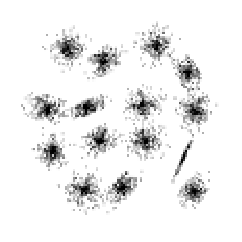
\includegraphics[keepaspectratio=true,scale=1]
{figuras/birch.eps}
\caption{Conjunto de Dados Sintético - \citeonline{birch}}
\label{data_titatic}
\end{figure}

\section{Protótipo}
Para realizar os testes comparativos um protótipo foi desenvolvido em C++ utilizando a plataforma \textit{C++ Builder XE2} da Embarcadero. O software carrega um arquivo csv do disco rígido que possui as informações dos dados a serem agrupados. É possível parametrizar ambos algoritmos através da interface, as janelas de parametrização podem ser vistas nas figuras 26 e 27. No centro do protótipo existem duas tabelas, uma para cada algoritmo. Nesta tabela são registrados os valores da entrada, a posição do neurônio vencedor que classificou as amostras e o erro desssa classificação. A visão geral do protótipo está na figura 25. 

\begin{figure}[!h]
\centering
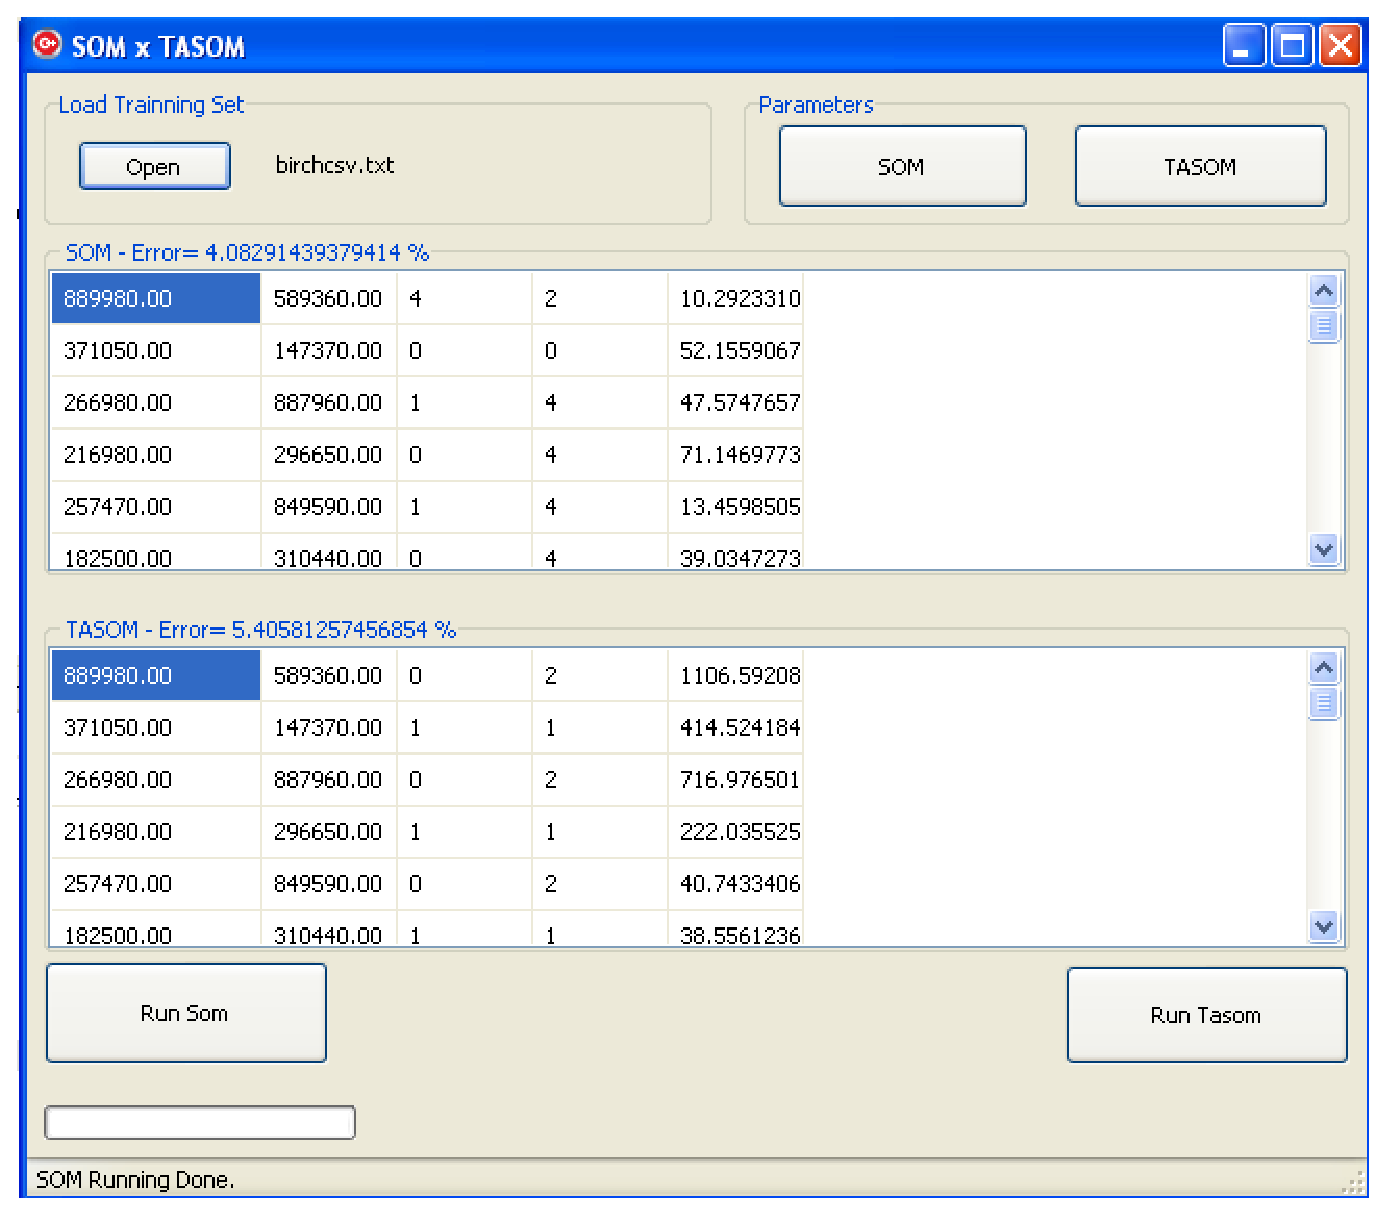
\includegraphics[keepaspectratio=true,scale=0.5]
{figuras/proto.eps}
\caption{Protótipo}
\label{data_titatic}
\end{figure}

\begin{figure}[!h]
\centering
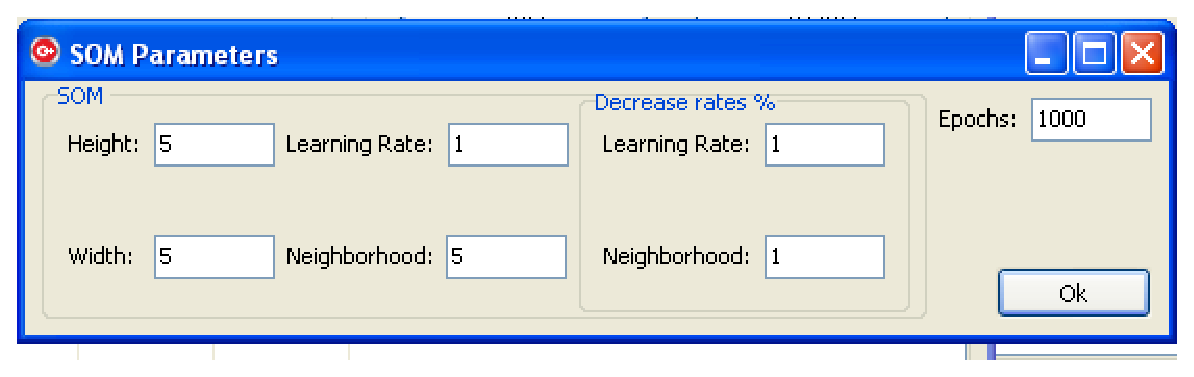
\includegraphics[keepaspectratio=true,scale=0.5]
{figuras/somparams.eps}
\caption{Parâmetros do SOM}
\label{data_titatic}
\end{figure}

\begin{figure}[!h]
\centering
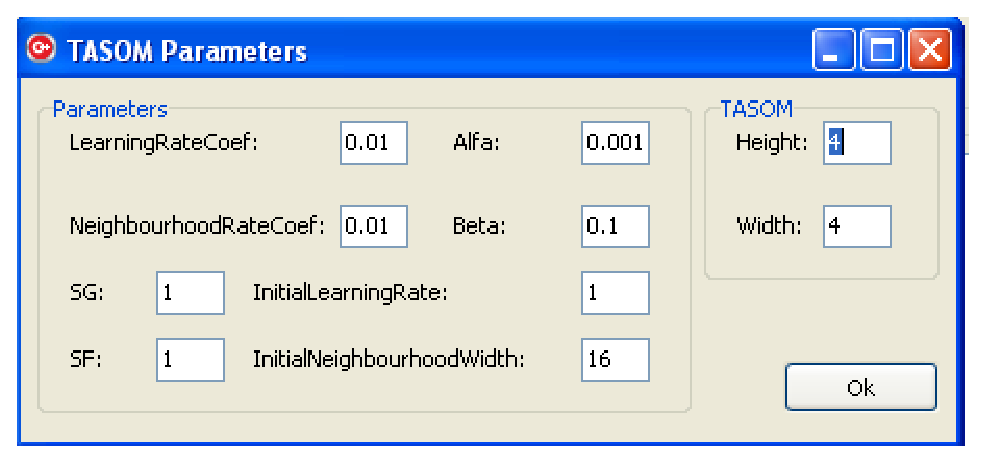
\includegraphics[keepaspectratio=true,scale=0.5]
{figuras/tasomparams.eps}
\caption{Parâmetros do TASOM}
\label{data_titatic}
\end{figure}

\section{SOM x TASOM}
Para comparar o SOM com o TASOM é necessário utilizar o mesmo contexto de aplicação. O algoritmo SOM não funciona em ambientes incrementais, o objetivo desta comparação é verificar se o desempenho do TASOM é aceitável também em ambiente não incremental. O conjunto de dados sintéticos apresentado anteriormente foi utilizado nas duas redes. As entradas foram randomicamente embaralhadas para que todos os agrupamentos sejam considerados como estando no mesmo espaço vetorial. Quando os agrupamentos são apresentados um de cada vez existem vários espaços vetoriais que mudam rapidamente e não um espaço com vários agrupamentos. Dentro dos dois algoritmos foi feita uma normalização, onde todas as entradas de todas as dimensões variam entre 0 e 1000. Esse intervalo de normalização foi escolhido pelo fato de o TASOM não se comportar bem com o intervalo padrão entre 0 e 1.

O algoritmo SOM foi treinado com 1000 épocas. Os critérios de parada do treinamento foram: A conclusão das mil épocas de treino ou, a taxa de aprendizado alcançar o valor zero ou o erro imediato da rede for menor que 10\%. Em todos os testes realizados o primeiro critério de parada alcançado foram as 1000 épocas, a taxa de aprendizado sempre ficou próxima de $5 x 10^{-5}$ em todos os testes. O conjunto de parâmetros escolhido para o SOM foram os que apresentaram menor erro final, eles foram configurados da seguinte forma: 

\begin{enumerate}
\item Altura do Mapa: 4.
\item Largura do Mapa: 4.
\item Raio de Vizinhança Inicial: 4.
\item Taxa de Aprendizagem Inicial: 1.
\item Decaimento da Taxa de Aprendizagem: 1\%.
\item Decaimento do Raio de Vizinhança: 1\%.
\end{enumerate}

As figuras 28, 29 e 30 mostram o estado da rede SOM em três momentos diferentes: Começo, metade e final do treino. Os pontos representam as amostras de entrada e os quadrados representam os neurônios da rede. É possível observar o desenvolvimento da aprendizagem ao decorrer do tempo, pois os neurônios se aproximam dos agrupamentos. Na figura 30 os pontos são coloridos de acordo com a cor do neurônio que os classifica.

\begin{figure}[!h]
\centering
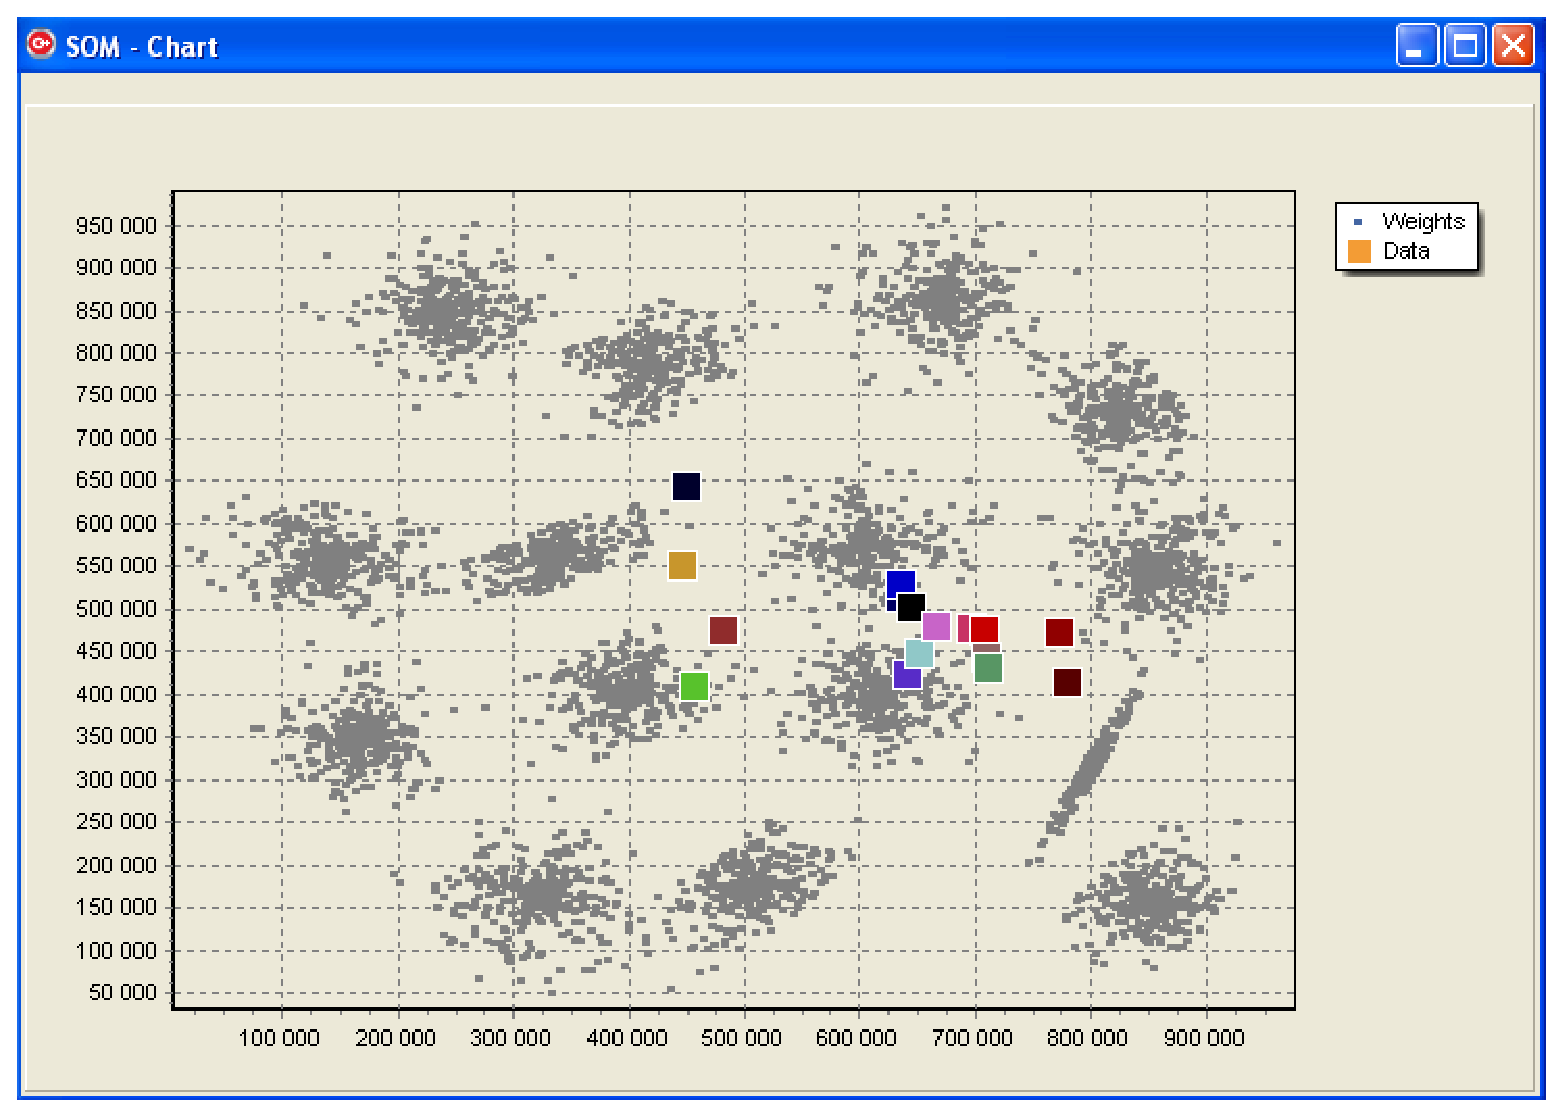
\includegraphics[keepaspectratio=true,scale=0.5]
{figuras/som1.eps}
\caption{Começo do Treinamento}
\label{data_titatic}
\end{figure} 


\begin{figure}[!h]
\centering
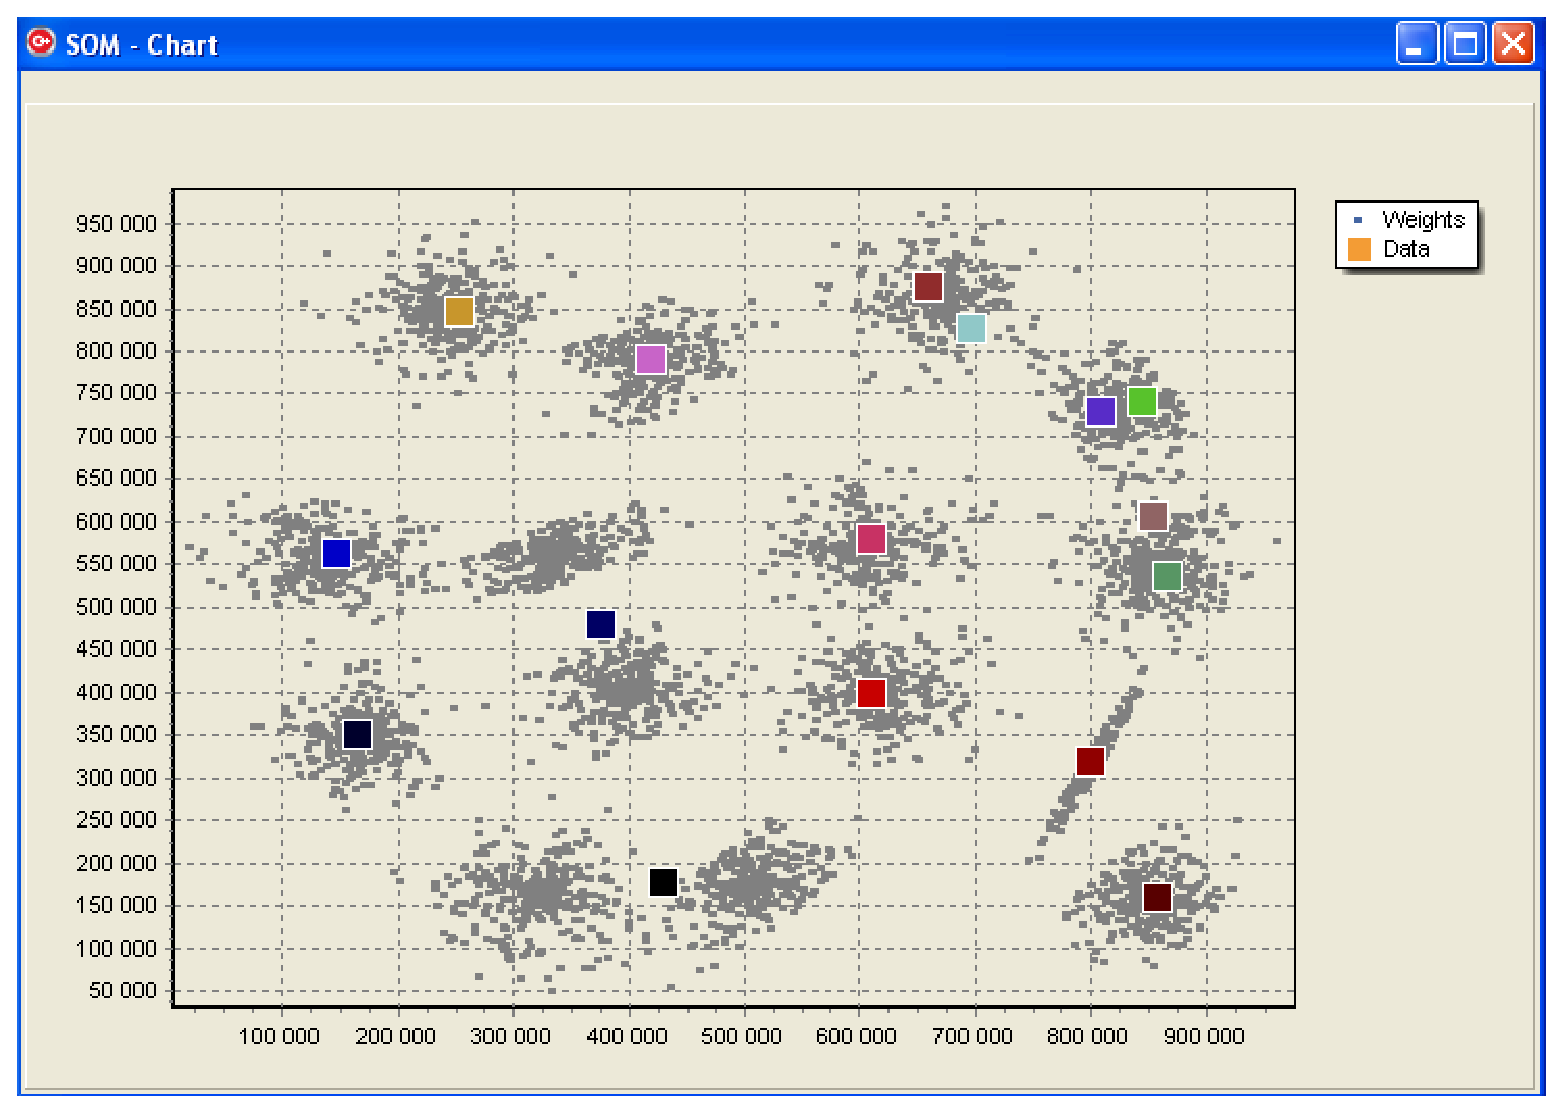
\includegraphics[keepaspectratio=true,scale=0.5]
{figuras/som2.eps}
\caption{Meio do Treinamento}
\label{data_titatic}
\end{figure} 


\begin{figure}[!h]
\centering
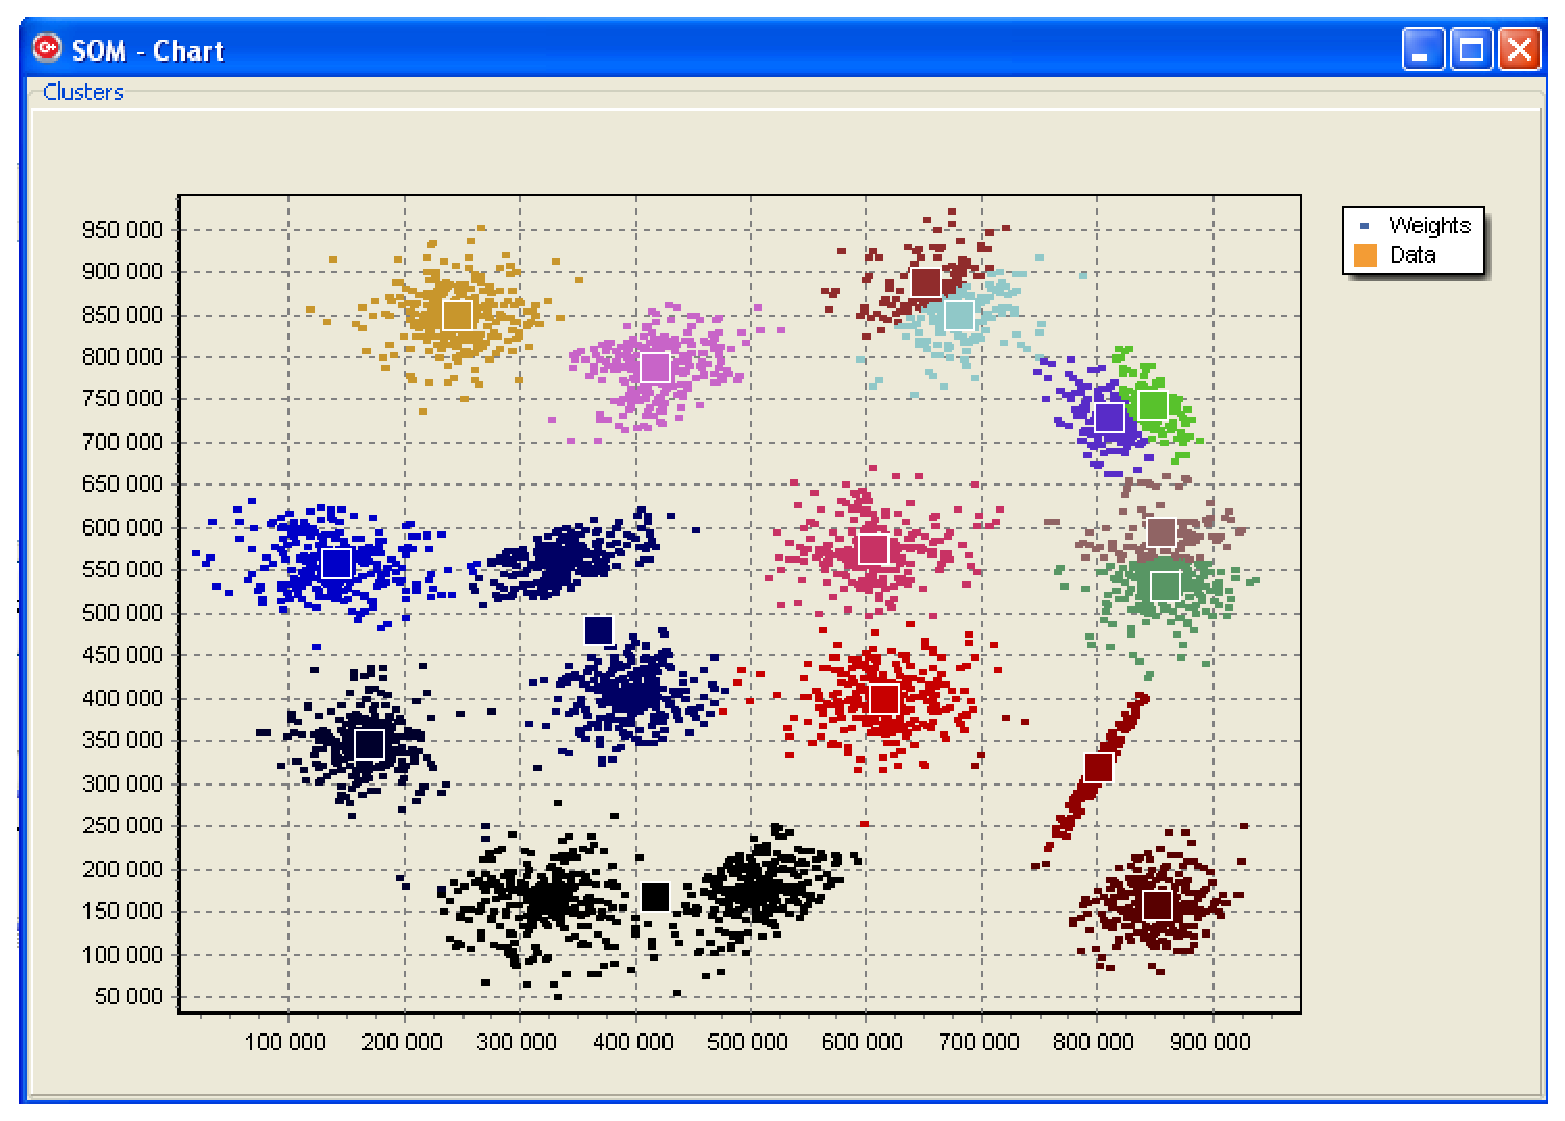
\includegraphics[keepaspectratio=true,scale=0.5]
{figuras/som3.eps}
\caption{Fim do Treinamento}
\label{data_titatic}
\end{figure} 

Por ser um algoritmo incremental o TASOM não possui fase de treinamento. O mapa se ajusta de acordo com as entradas que chegam ao sistema. O conjunto de parâmetros escolhidos para o TASOM foram os que fizeram com o que mapa apresentasse menor erro final, eles foram configurados da seguinte forma: 

\begin{enumerate}
\item Altura do Mapa: 4.
\item Largura do Mapa: 4.
\item Raio de Vizinhança Inicial: 4.
\item Taxa de Aprendizagem Inicial: 1.
\item Coeficiente de Aprendizagem: 0.01.
\item Coeficiente de Vizinhança: 0.01.
\item SG: 1.
\item SF: 1.
\item Alfa: 0.001.
\item Beta: 0.1.
\end{enumerate}


As figuras 31, 32 e 33 mostram o estado da rede TASOM em três momentos diferentes: Começo, metade e final da apresentação. Os pontos representam as amostras de entrada e os quadrados representam os neurônios da rede. É possível observar o desenvolvimento da aprendizagem ao decorrer do tempo, pois os neurônios se aproximam dos agrupamentos. Em todas as etapas as entradas já são coloridas de acordo com os neurônios que as classificam. A execução do TASOM é mais rápida do que a do SOM. Considerando somente o número de vezes que o conjunto de entrada é apresentado, o TASOM se mostrou 1000 vezes mais rápido, pois os dados de entrada são apresentados apenas uma vez.


\begin{figure}[!h]
\centering
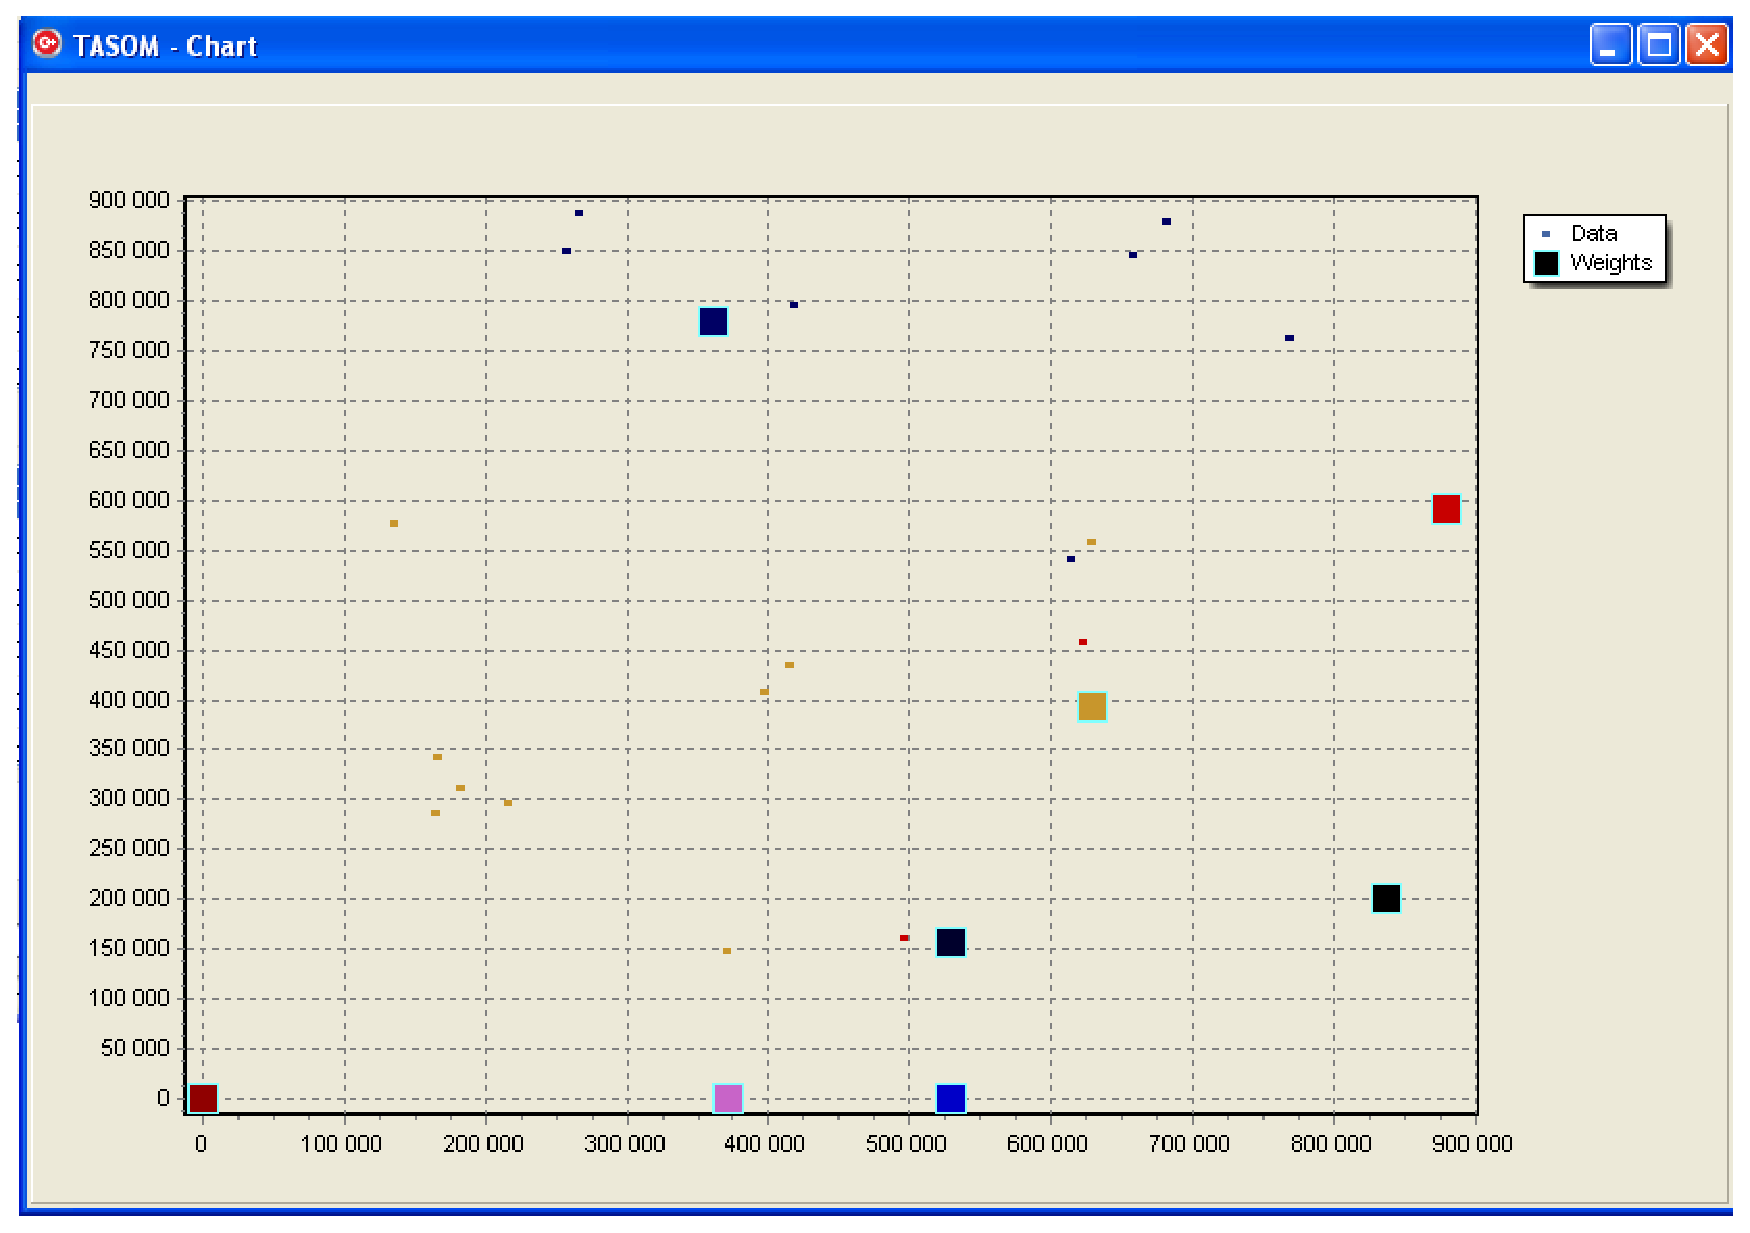
\includegraphics[keepaspectratio=true,scale=0.5]
{figuras/tasom1.eps}
\caption{Começo - Estático}
\label{data_titatic}
\end{figure}  

\begin{figure}[!h]
\centering
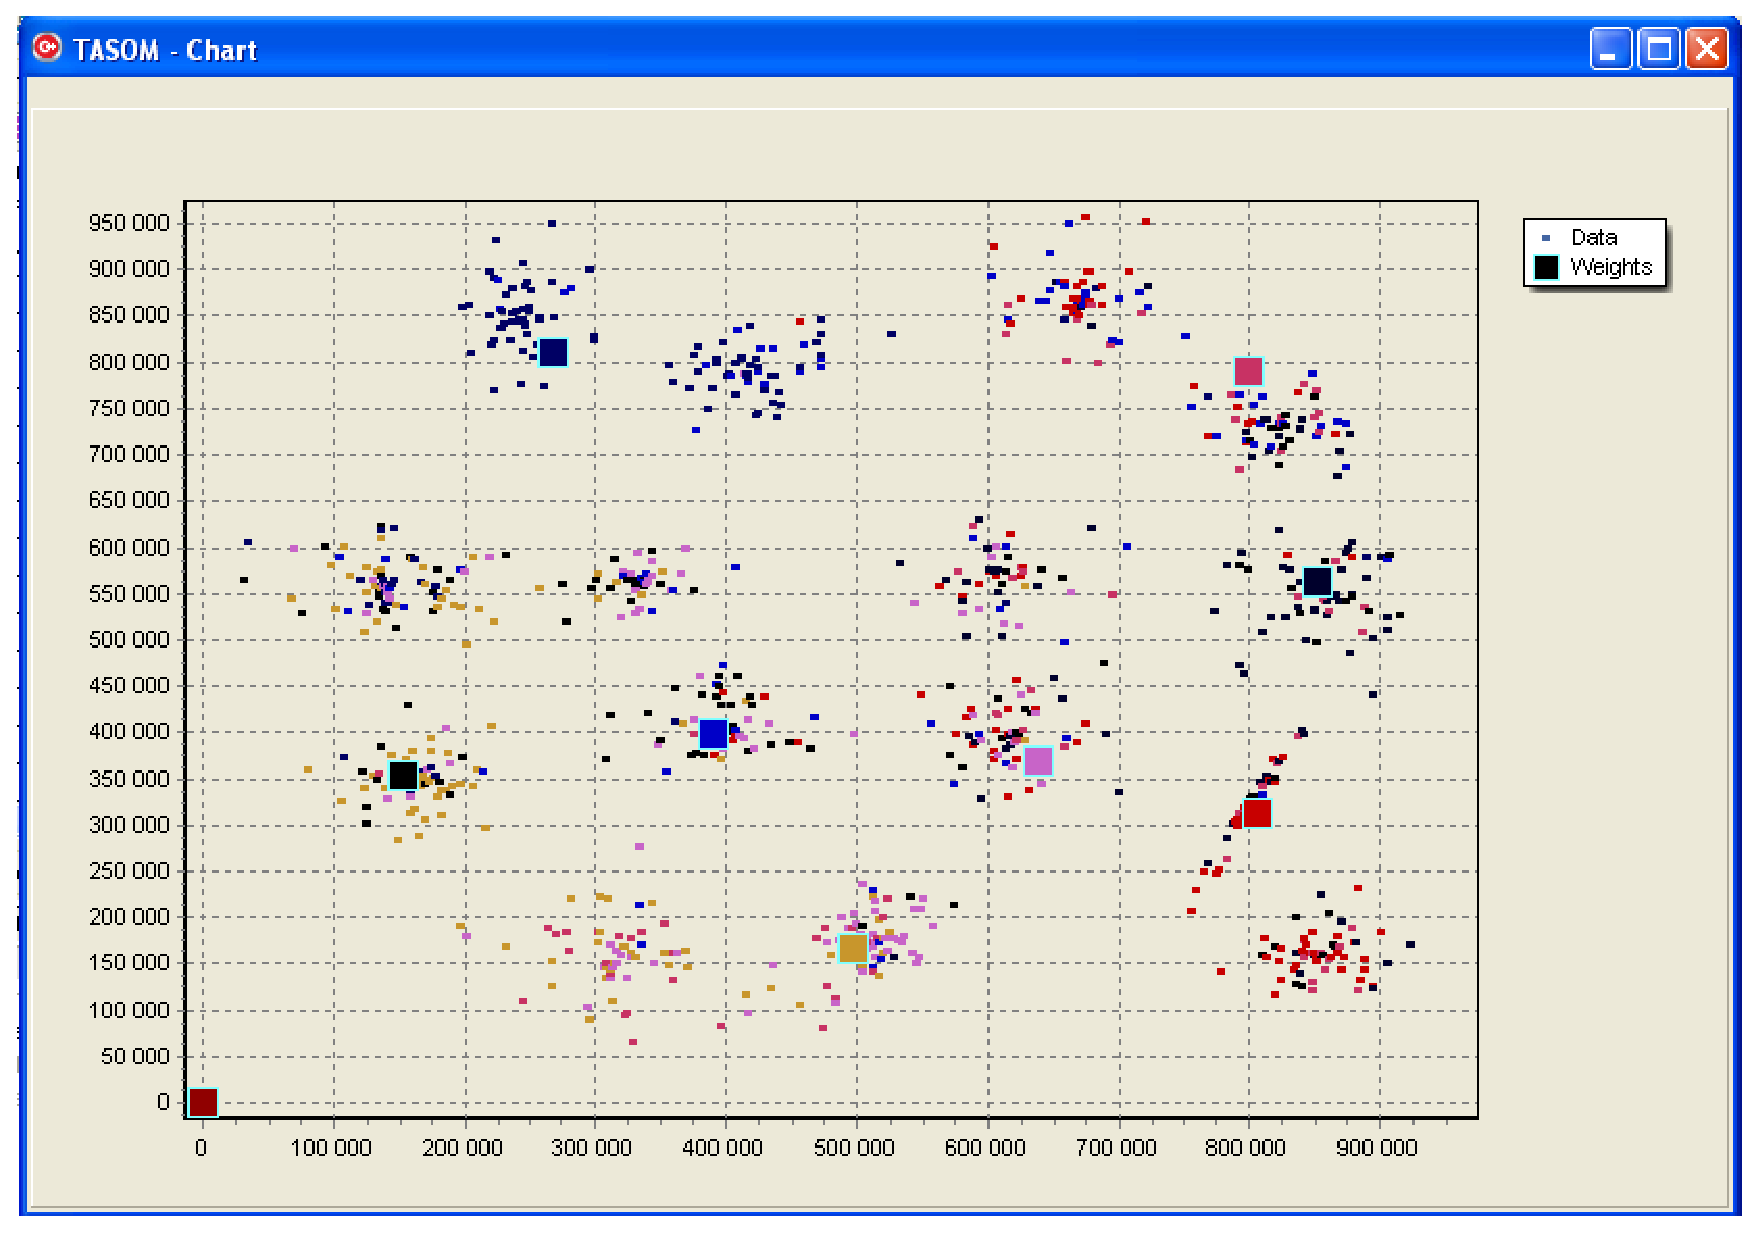
\includegraphics[keepaspectratio=true,scale=0.5]
{figuras/tasom2.eps}
\caption{Meio - Estático}
\label{data_titatic}
\end{figure}

\begin{figure}[!h]
\centering
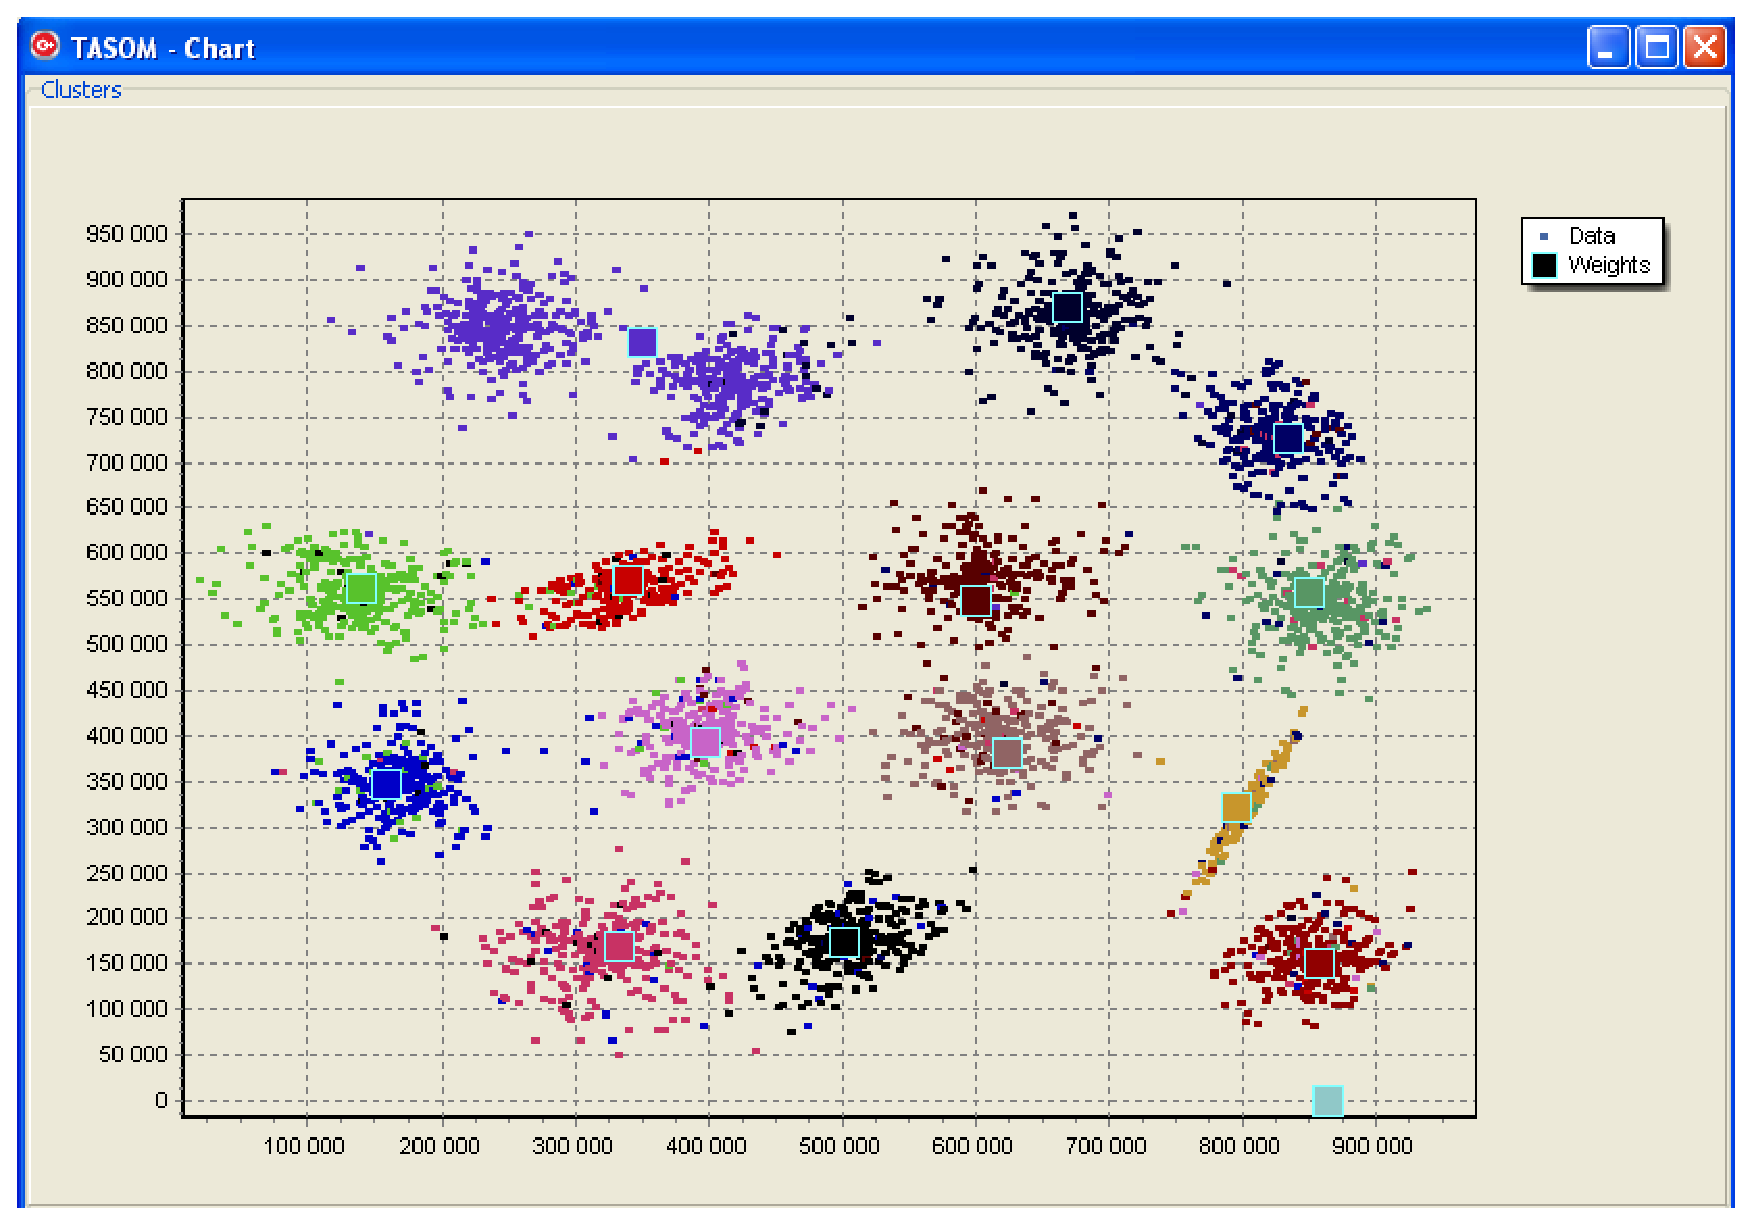
\includegraphics[keepaspectratio=true,scale=0.5]
{figuras/tasom3.eps}
\caption{Fim - Estático}
\label{data_titatic}
\end{figure}  

Para comparar os dois algoritmos é necessário estabelecer uma métrica que seja aplicável aos dois mapas. Para verificar a capacidade que cada algoritmo tem em corretamente agrupar os conjuntos corretos, foi utilizado o erro médio final. O erro final é a distância entre a entrada e o neurônio que a classificou depois da estabilização da rede. Após todas as épocas de treinamento do SOM e depois de todas as amostras passarem pelo TASOM, as entradas foram novamente apresentadas e foi possível calcular o erro médio em um momento em que ambos os mapas estão estabilizados. Foram feitas 10 execuções, pois ambas as redes possuem uma inicialização de pesos randômica que pode influenciar no resultado final. A tabela 3 mostra o erro médio de cada um dos algoritmos.

\begin{table}[h]
\centering
\caption{SOM x TASOM}
\label{comp}
\begin{tabular}{c|l|l|}
\cline{2-3}
                            & SOM      & TASOM    \\ \hline
\multicolumn{1}{|c|}{1}     & 5.134363\% & 4.675699\% \\ \hline
\multicolumn{1}{|c|}{2}     & 5.134363\% & 7.970087\% \\ \hline
\multicolumn{1}{|c|}{3}     & 5.134363\% & 4.657833\% \\ \hline
\multicolumn{1}{|c|}{4}     & 5.134363\% & 4.636273\% \\ \hline
\multicolumn{1}{|c|}{5}     & 5.134363\% & 6.346224\% \\ \hline
\multicolumn{1}{|c|}{6}     & 5.134363\% & 3.632400\% \\ \hline
\multicolumn{1}{|c|}{7}     & 5.134363\% & 3.755198\% \\ \hline
\multicolumn{1}{|c|}{8}     & 5.134363\% & 4.669887\% \\ \hline
\multicolumn{1}{|c|}{9}     & 5.134363\% & 3.695024\% \\ \hline
\multicolumn{1}{|c|}{10}    & 5.134363\% & 4.780292\% \\ \hline
\multicolumn{1}{|l|}{Média} & 5.134363\% & 4.881891\% \\ \hline
\end{tabular}
\end{table}

\section{TASOM em Ambiente Incremental}
Para medir a eficiência do TASOM em um ambiente incremental de maneira sintética é necessário utilizar um conjunto de entradas que muda bruscamente. Dessa forma é possível verificar se o TASOM é capaz de aprender novos conceitos com rapidez e eficiência. O cálculo de erro neste caso só deve levar em consideração a distância entre o neurônio e a entrada na hora em que o dado é apresentado, pois amostras subsequentes podem introduzir novos conceitos que serão absorvidos por aquele neurônio. O mesmo conjunto de entradas foi utilizado, mas seus agrupamentos são apresentados de maneira sequencial. Para realizar este teste todos os parâmetros da rede TASOM previamente apresentados foram mantidos. As figuras 34, 35 e 36 são representações no começo, meio e fim da apresentação do dados de entrada.

\begin{figure}[!h]
\centering
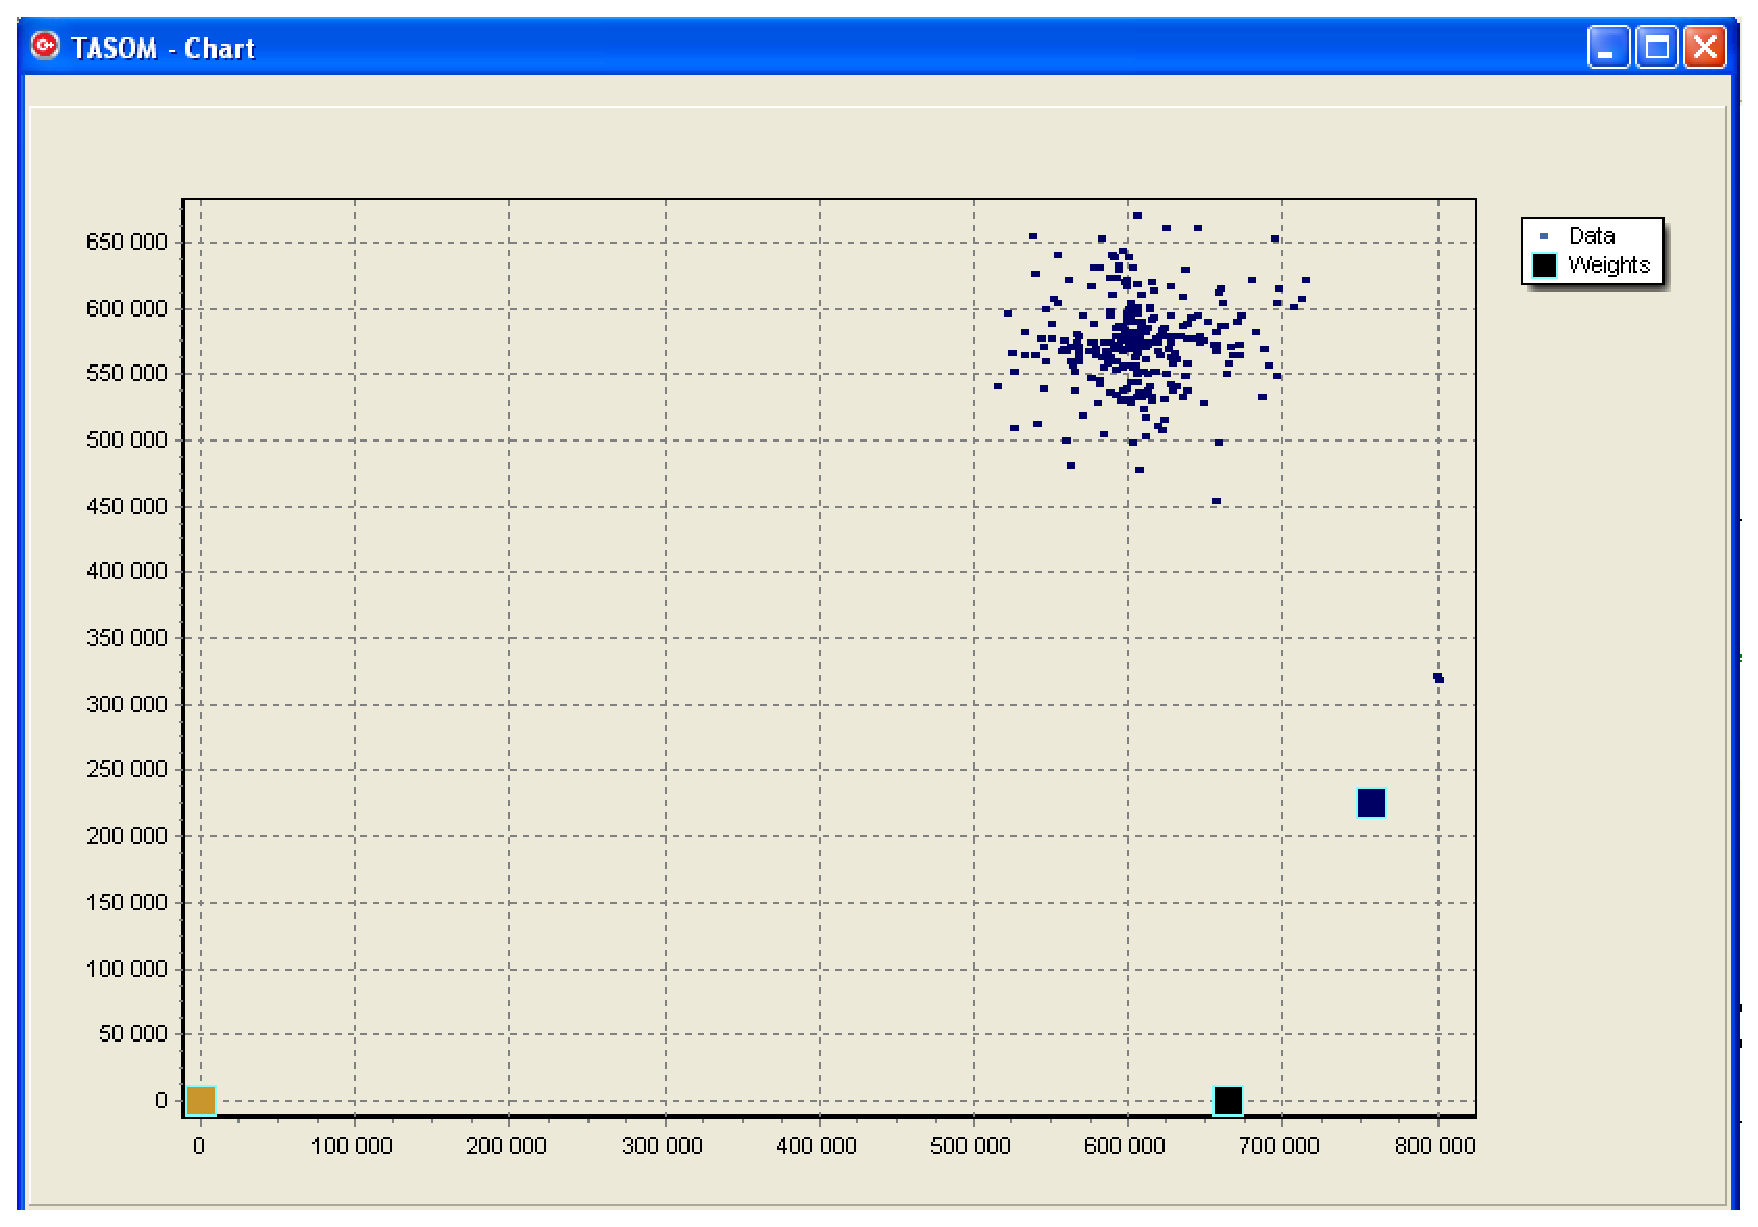
\includegraphics[keepaspectratio=true,scale=0.5]
{figuras/tsom1.eps}
\caption{Começo - Dinâmico}
\label{data_titatic}
\end{figure}  

\begin{figure}[!h]
\centering
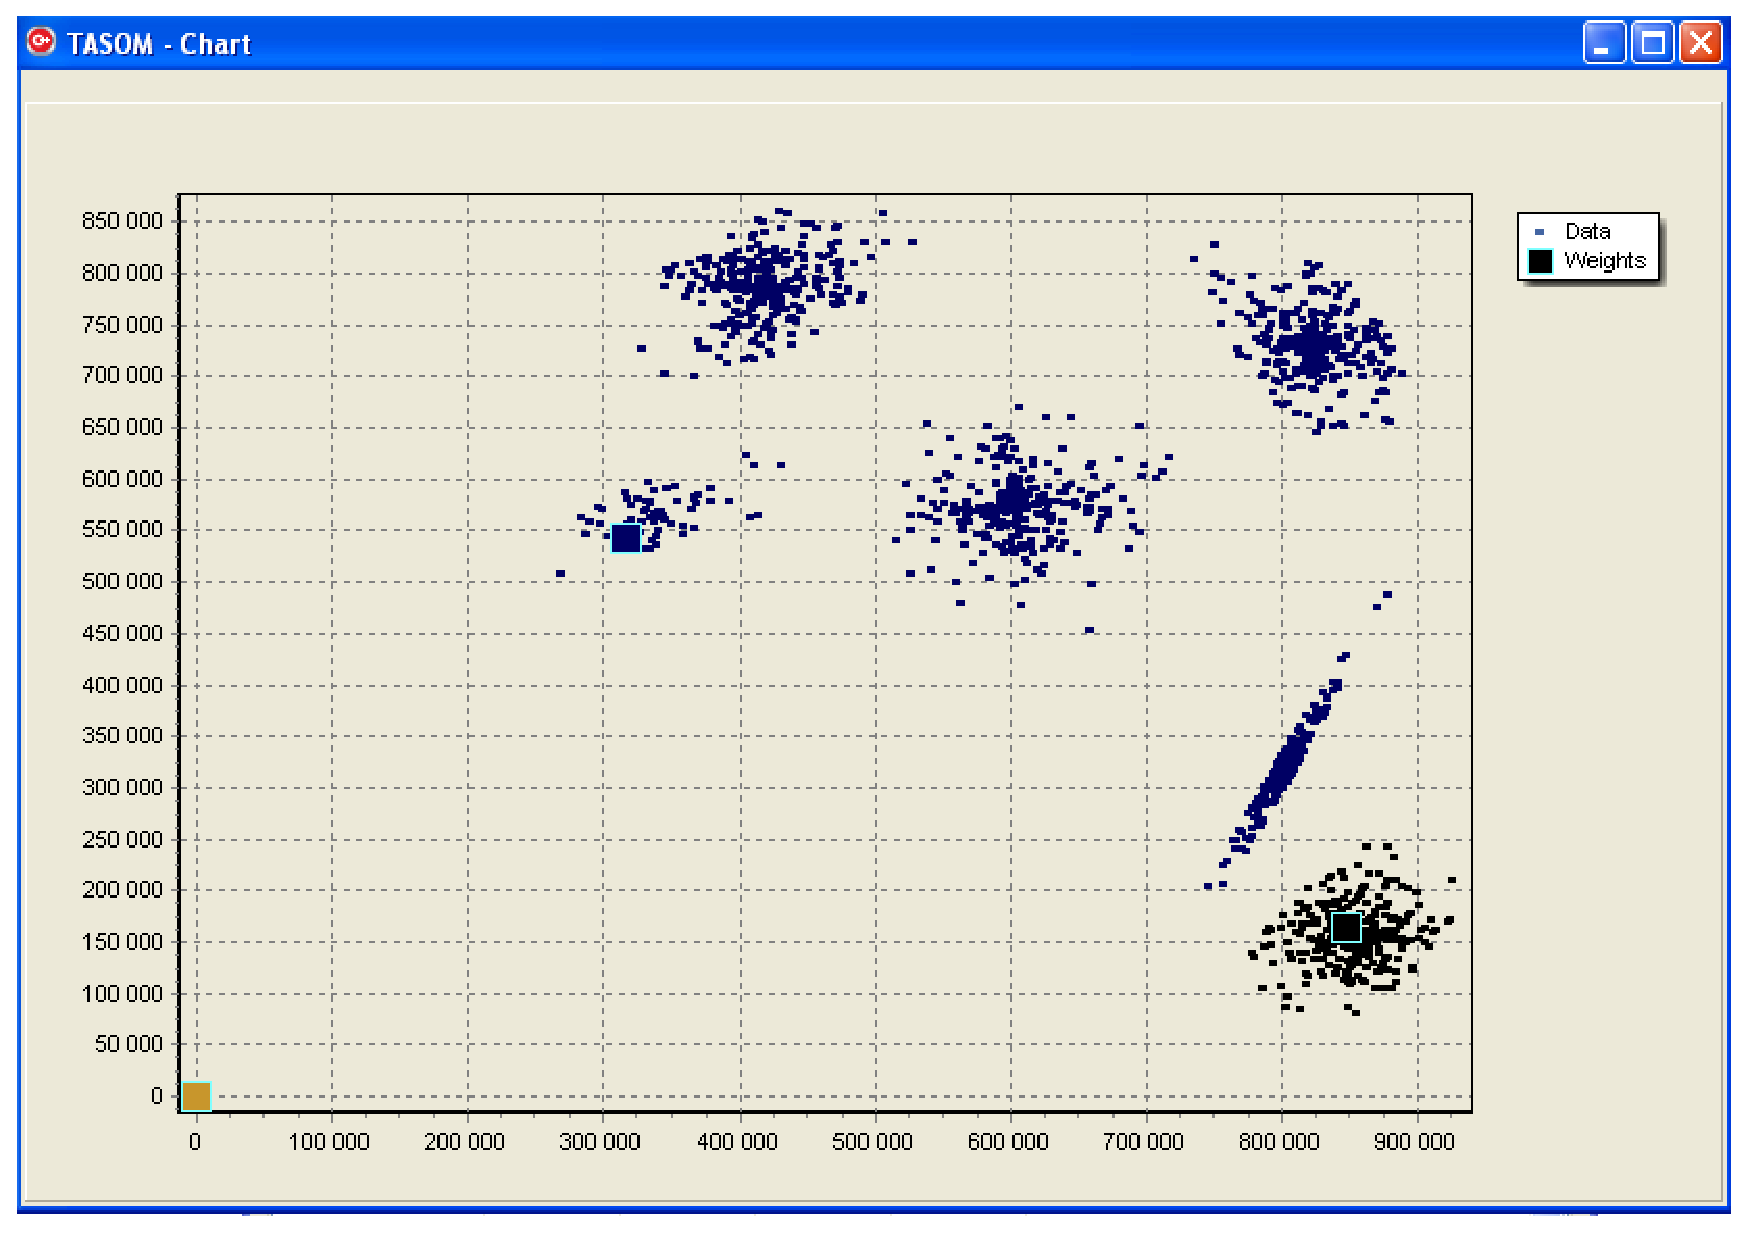
\includegraphics[keepaspectratio=true,scale=0.5]
{figuras/tsom2.eps}
\caption{Meio - Dinâmico}
\label{data_titatic}
\end{figure}

\begin{figure}[!h]
\centering
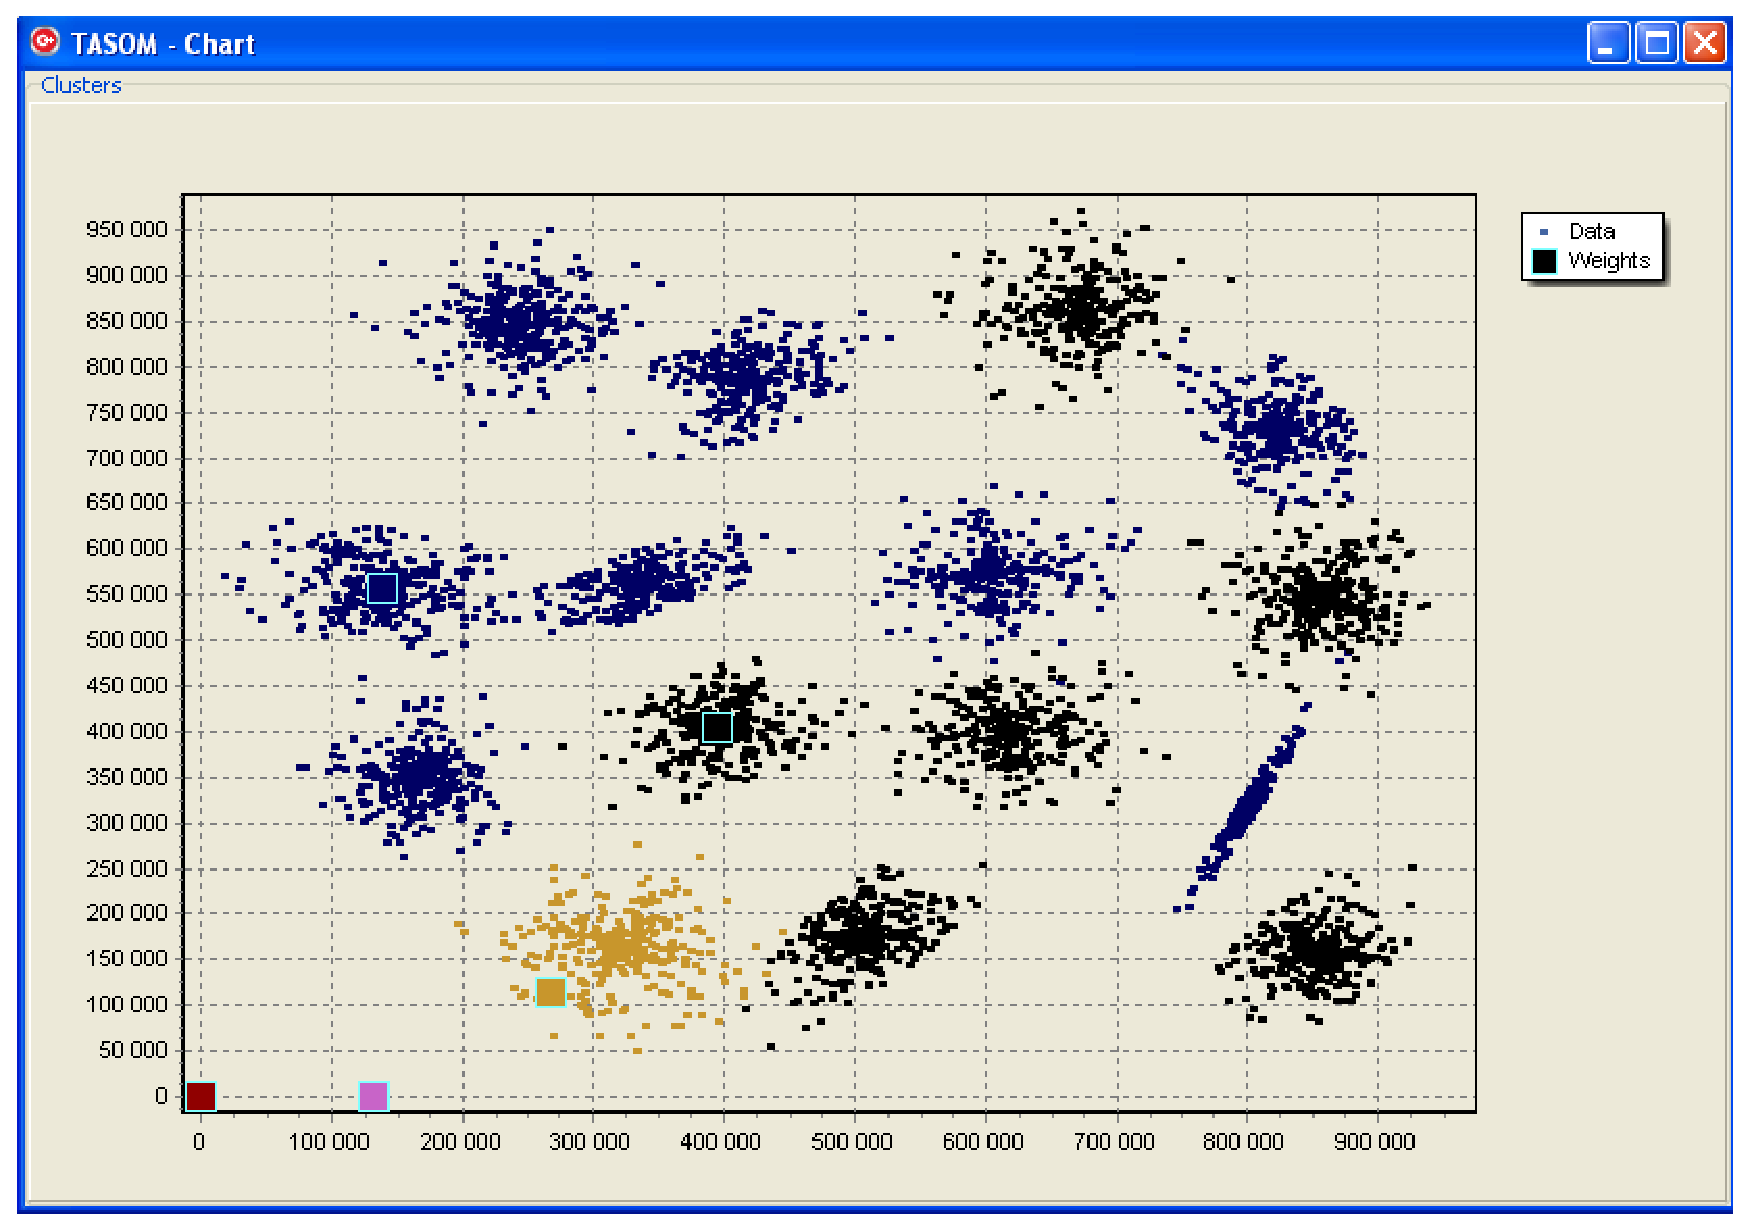
\includegraphics[keepaspectratio=true,scale=0.5]
{figuras/tsom3.eps}
\caption{Fim - Dinâmico}
\label{data_titatic}
\end{figure}

\begin{table}[h]
\centering
\caption{TASOM Incremental}
\label{my-label}
\begin{tabular}{c|l|}
\cline{2-2}
                            & TASOM      \\ \hline
\multicolumn{1}{|c|}{1}     & 11.454104\%  \\ \hline
\multicolumn{1}{|c|}{2}     & 11.122445\%  \\ \hline
\multicolumn{1}{|c|}{3}     & 6.6950870\%  \\ \hline
\multicolumn{1}{|c|}{4}     & 5.5194768\%  \\ \hline
\multicolumn{1}{|c|}{5}     & 11.454104\%  \\ \hline
\multicolumn{1}{|c|}{6}     & 11.563024\% \\ \hline
\multicolumn{1}{|c|}{7}     & 5.1994760\%  \\ \hline
\multicolumn{1}{|c|}{8}     & 4.6800620\%  \\ \hline
\multicolumn{1}{|c|}{9}     & 4.6800621\%  \\ \hline
\multicolumn{1}{|c|}{10}    & 4.9833902\%   \\ \hline
\multicolumn{1}{|l|}{Média} & 7.7351230\% \\ \hline
\end{tabular}
\end{table} 

É possível observar que cada um dos agrupamentos é marcado por apenas um neurônio. Isso acontece porque o neurônio mais próximo a primeira amostra apresentada de cada conjunto se move até a posição daquele agrupamento. Depois disso ele sempre é o neurônio que está mais próximo daquele grupo. O TASOM é altamente sensível aos pesos randômicos de inicialização, é possível observar esse fenômeno quando a quantidade de neurônios agrupadores muda de execução para execução e na variação de erro que foi observada na comparação entre o SOM e o TASOM. O erro encontrado para este teste pode ser observado na tabela 4.

\section{Resultado da Comparação}
O TASOM foi capaz de superar o SOM em ambiente estático, apresentando um erro médio de 4.881891\% contra 5.134363\% do SOM. Em um contexto incremental o erro médio foi de 7.7351230\%. Os resultados destes experimentos indicam que o TASOM é uma boa alternativa ao SOM, pois é capaz de gerar um mapa que possui as mesmas características do SOM e é capaz de ser usado em um contexto incremental. Alguns cuidados devem ser tomados no uso do TASOM, a escolha dos parâmetros inicias pode ser ser complicada e ele é muito sensível a semente inicial dos pesos.

























